\section*{Introduction}
Dans ce chapitre, nous observerons les différentes avancées qui ont déjà eu lieu dans le domaine de la transcription automatique de la musique et de la batterie afin de situer notre démarche.\\
Nous aborderons le passage crucial du monophonique au polyphonique dans la transcription. Nous ferons un point sur les deux grandes parties de l’AMT de bout en bout : de l’audio vers le MIDI puis des données MIDI vers l’écriture d’une partition. Ensuite, nous discuterons des approches linéaires et des approches hiérarchiques.
\section{Monophonique et polyphonique}
Les premiers travaux ont été faits sur l’identification des instruments monophoniques\footnote{Instruments produisant une note à la fois, ou plusieurs notes de même durée (monophonie par accord).} \cite{future_directions}. Actuellement, le problème de l'estimation automatique de la hauteur des signaux monophoniques peut être considéré comme résolu, mais dans la plupart des contextes musicaux, les instruments sont polyphoniques. L'estimation des hauteurs multiples (détection multi-pitchs ou F0 multiples) est le problème central de la création d'un système de transcription de musique polyphonique. Il s’agit de la détection de notes qui peuvent apparaître simultanément et être produites par plusieurs instruments différents. Ce défi est donc majeur pour la batterie puisque c’est un instrument qui est lui-même constitué de plusieurs instruments (caisse-claire, grosse-caisse, cymbales, toms, etc…). Le fort degré de chevauchement entre les durées ainsi qu’entre les fréquences complique l’identification des instruments polyphoniques. Cette tâche est étroitement liée à la séparation des sources et concerne aussi la séparation des voix. Les performances des systèmes actuels ne sont pas encore suffisantes pour permettre la création d'un système automatisé capable de transcrire de la musique polyphonique sans restrictions sur le degré de polyphonie ou le type d'instrument. Cette question reste donc encore ouverte. 
\section{Audio vers MIDI}
%\textit{Utilité de l’audio vers MIDI dans la vraie vie $\Rightarrow$ p. 4 et 5 de \cite{Review_ADT}.}\\\\
Jusqu’à aujourd’hui, les recherches se sont majoritairement concentrées sur le traitement du signal vers la génération du MIDI \cite{AMT_for_2_Instru}. Cette partie englobe plusieurs sous-tâches dont la détection multi-pitchs, la détection des onset et des offset, l'estimation du tempo, la quantification du rythme, la classification des genres musicaux, etc…\\
En ADT \cite{Review_ADT}, plusieurs stratégies de répartition pré/post-processing sont possibles pour la détection multi-pitchs. Entamer la détection dès le pré-processing, en supprimant les features non-pertinentes pendant la séparation des sources afin d’obtenir une meilleure détection des instruments de la batterie, est une démarche intuitive : supprimer la structure harmonique pour atténuer l’influence des instruments à hauteurs sur la détection grosse-caisse et caisse-claire en est un exemple. Mais certaines études montrent que des expériences similaires ont donné des résultats non-concluants et que la suppression des instruments à hauteurs peut avoir des effets néfastes sur les performances de l’ADT. En outre, les systèmes d’ADT basés sur des RNN ou des NMF font la séparation des sources pendant l’optimisation, ce qui réduit la nécessité de la faire pendant le pré-processing.\\
Pour la reconnaissance des instruments, une approche possible \cite{Eronen} est de mettre un modèle probabiliste dans l’étape de la classification des évènements afin de classer les différents sons de la batterie. Cette méthode permet de se passer de samples audio isolés en modélisant la progression temporelle des features avec un HMM. Les features sont transformés en représentations statistiques indépendantes.
L’approche AdaMa \cite{adama_1} est une autre approche de la même catégorie ; elle commence par une estimation initiale des sons de la batterie qui sont itérativement raffinés pour correspondre à (pour matcher) l’enregistrement visé.\\
%- Extraction of rhythmic information (tempo, beat, and musical timing)\\
\section{MIDI vers partition}
Le plus souvent, lorsque les articles abordent la transcription automatique de bout en bout (de l’audio à la partition), l’appellation « score » (\textit{partition}) désigne un ouput au format Music XML, ou simplement MIDI. Par exemple, dans \cite{SHIBATA2021262}, la chaîne de traitement va jusqu’à la génération d’une séquence MIDI quantifiée qui est importée dans MuseScore pour en extraire manuellement un fichier MusicXML contenant plusieurs voix.\\
Seuls quelques travaux récents s’intéressent de près à la création d’outils permettant la génération de partition. Le problème de la conversion d'une séquence d'évènements musicaux symboliques en une partition musicale structurée est traité notamment dans \cite{foscarin:hal-01988990}. Ce travail, qui vise à résoudre en une fois la quantification du rythme et la production de partition, s’appuie tout au long du processus sur  des grammaires génératives qui fournissent un modèle hiérarchique \textit{a priori} des partitions. Les expériences ont des résultats prometteurs, mais il faut relever qu’elle ont été menées avec un ensemble de données composé d'extraits monophoniques ; il reste donc à traiter le passage au polyphonique en couplant le problème de la séparation des voix avec la quantification du rythme.\\
L'approche de \cite{foscarin:hal-01988990} est fondée sur la conviction que la complexité de la structure musicale dépasse les modèles linéaires.
\section{Approche linéaire et approche hiérarchique}
Plusieurs travaux ont d’abord privilégié l’approche stochastique. Par exemple, Shibata \textit{et al.} \cite{SHIBATA2021262} ont utilisé le modèle de Markov caché (HMM)\footnote{\url{https://fr.wikipedia.org/wiki/Modèle_de_Markov_caché}\\\url{https://en.wikipedia.org/wiki/Hidden_Markov_model}} pour la reconnaissance de la métrique. Les auteurs utilisent d’abord deux réseaux de neurones profonds, l’un pour la reconnaissance des pitchs et l’autre pour la reconnaissance de la vélocité. Pour la dernière couche, la probabilité est obtenue par une fonction sigmoïde. Ils construisent ensuite plusieurs HMM métriques étendus pour la musique polyphonique correspondant à des métriques possibles, puis ils calculent la probalitité maximale pour chaque modèle afin d’obtenir la métrique la plus probable.\newpage
\begin{figure}[h]
	\centering
	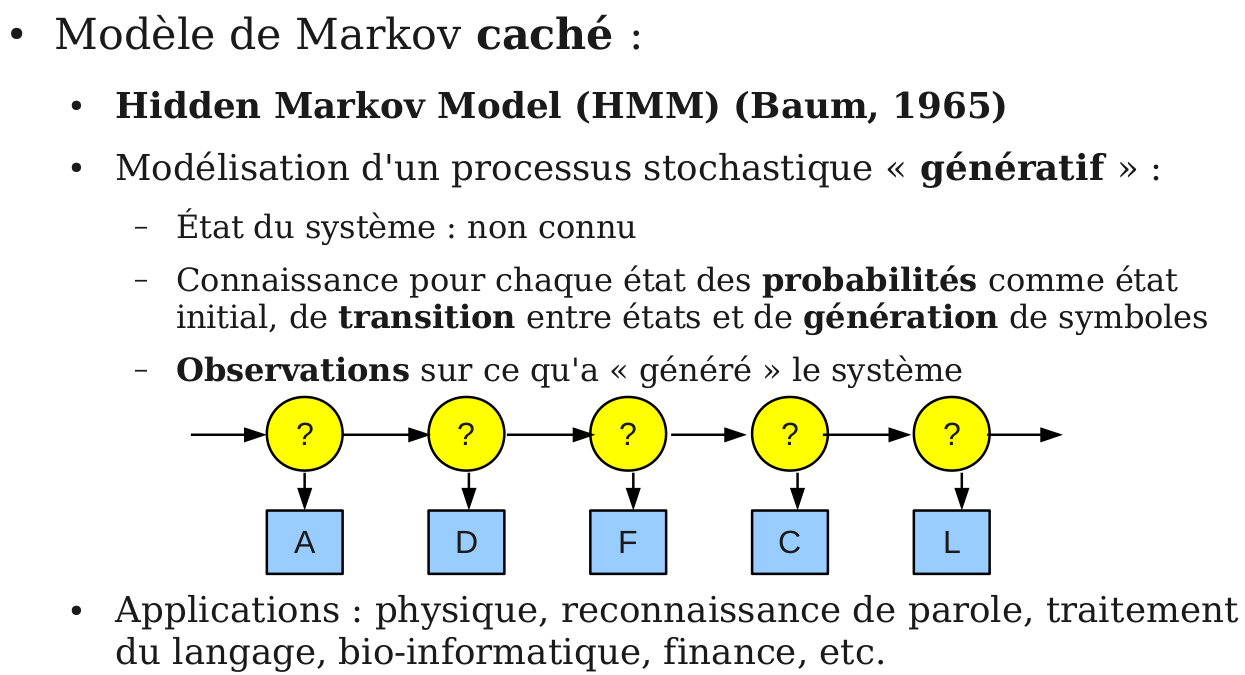
\includegraphics[height=50mm, width=90mm]{z_images/2_etat_de_l_art/0_hmm.png}
	\caption{HMM}
\end{figure}
\textit{Source : Cours de Damien Nouvel\footnote{\url{https://damien.nouvels.net/fr/enseignement}}}\\\\
L’évaluation finale des résultats de \cite{SHIBATA2021262} montre qu’il faut rediriger l’attention vers les valeurs des notes, la séparation des voix et d'autres éléments délicats de la partition musicale qui sont significatifs pour l'exécution de la musique. Or, même si la quantification du rythme se fait le plus souvent par la manipulation de données linéaires allant notamment des \textit{real time units} (secondes) vers les musical \textit{time units} (temps, métrique,…), de nombreux travaux suggèrent d’utiliser une approche hiérarchique puisque le langage musical est lui-même structuré.\\
En effet, l’usage d’arbres syntaxiques est idéale pour représenter le langage musical. Une méthodologie simple pour la description et l'affichage des structures musicales est présentée dans \cite{rythm_tree}. Les RT y sont évoqués comme permettant une cohésion complète de la notation musicale traditionnelle avec des notations plus complexes. Jacquemard \textit{et al.} \cite{jacquemard:hal-01134096} propose aussi une représentation formelle du rythme, inspirée de modèles théoriques antérieurs et dont l’objectif est la réécriture de termes. Ils démontrent aussi l’application des arbres de rythmes pour les équivalences rythmiques dans \cite{jacquemard:hal-01403982}. La réécriture d’arbres, dans un contexte de composition assistée par ordinateur, par exemple, pourrait permettre de suggérer à un utilisateur diverses notations possibles pour une valeur rythmique, avec des complexités différentes.\\La nécessité d’une approche hiérarchique pour la production automatique de partition est évoquée dans \cite{foscarin:hal-01988990}. Les modèles de grammaire qui y sont exposés sont différents de modèles markoviens linéaires de précédents travaux.\newpage
\begin{figure}[h]
	\centering
	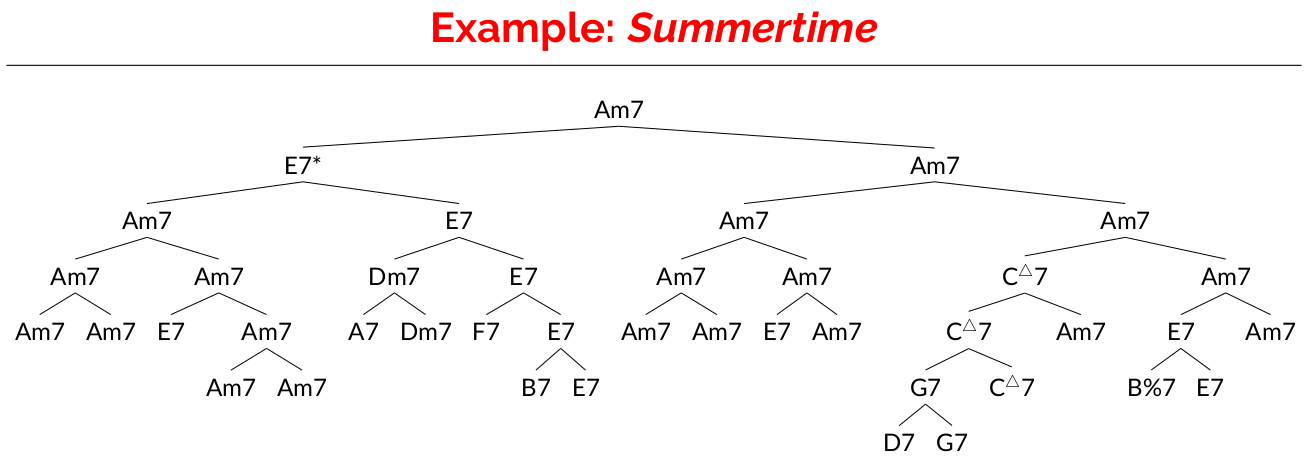
\includegraphics[height=40mm, width=120mm]{z_images/2_etat_de_l_art/1_summertime_tree.png}
	\caption{arbre\_jazz}
	\textit{Représentation arborescente d’une grille harmonique} \cite{harasimjazz}
\end{figure}
\section*{Conclusion}
La plupart des travaux déjà existants sur l’ADT ont été énumérés par Wu \textit{et al.} \cite{Review_ADT} qui, pour mieux comprendre la pratique des systèmes d’ADT, se concentrent sur les méthodes basées sur la factorisation matricielle non négative et celles utilisant des réseaux neuronaux récurrents. La majorité de ces recherches se concentre sur des méthodes de calcul pour la détection d'événements sonores de batterie à partir de signaux acoustiques ou sur la séparation entre les évènements sonores de batterie avec ceux des autres instruments dans un orchestre ou un groupe de musique \cite{2802}, ainsi que sur l'extraction de caractéristiques de bas niveau telles que la classe d'instrument et le moment de l'apparition du son. Très peu d'entre eux ont abordé la tâche de générer des partitions de batterie et, même quand le sujet est abordé, l’output final n’est souvent qu’un fichier MIDI ou MusicXML et non une partition écrite.\\
Il n’existe pas de formalisation de la notation de la batterie ni de réelle génération de partition finale, dont les enjeux principaux seraient :\\1) le passage du monophonique au polyphonique, comprenant la distinction entre les sons simultanés et les flas ou autres ornements ;\\2) les choix d’écritures spécifiques à la batterie concernant la séparation des voix et les continuations.